%!TEX root = ../dokumentation.tex

%TODO: Einleitungen überarbeiten

\chapter{Contribution}\label{cha:Contribution}

The proposed solution of this work is inspired by the approaches for compute shaders described in \autoref{section:computeApproaches}. The code for the shaders is written in a source language which supports the different methods for debugging listed in \autoref{paragraph:debuging} while running on the CPU.

To run the shader as usual on the GPU the shaders written in the source language is translated to the shader language and loaded on the hardware.

To enable the functionality while debugging, the linking of the shaders and the steps in between the shaders on the graphics pipeline, usually already provided by the graphics hardware, will be simulated in the source language.

\section{Steps for translating the shader code}
\label{section:contribution_translating}

In most cases the access of attributes within a shader is done by getting its location from its name.\myCite{Lighthouse3d.2013} To directly access the variables, a way to translate the shader from the source language keeping the variable names is chosen. As explained in \autoref{section:translating} by directly translating the language without compiling it to intermediate stages all kinds of languages can be chosen as source languages and the variable names can easily be retained.

Shaders within the graphics pipeline have a special way of being structured so the input and output within their respective stage is flowing correctly through the shader. Because of this the code written in the source language ment to be translated to a shader should mimic the structure the shader language provides. This means when the shader language provides certain structures for input or output or a specific point of entry into the code an equivalent for these has to be given in the code written in the source language.

The translation is done by converting the source language into a syntax tree from which the syntax will be extracted in the shader language. Occurances of variable types also have to be translated to their correct equivalent.

It has to be considered that specific syntax, like header lines or special accessors, only existing in the shader language has to be emulated in some way. Examples for this are shown in \autoref{cha:Implementation} for the translation of C\# to GLSL.

\section{Steps for simulating the graphics pipeline}
\label{section:contribution_simulating}

To simulate the graphics pipeline to be able to run and thereby debug the shaders written in the source language on the CPU the shaders have to be written in a structure that they can be inserted and exchanged within the simulated pipeline. The simulated pipeline has to implement the steps usually running automated on the GPU in between the different shader stages.

It is determined which kinds of shaders should be able to be simulated and therefore which parts of the pipeline as described in \autoref{paragraph:pipeline} have to be implemented.

\paragraph{Instance of a shader within the source language}

A shader in the source language should be contained within a fixed structure like a class. Thereby the execution of the shader within the simulated pipeline is easier managable compared to having to composite the shader out of multiple parts.
As already mentioned in \autoref{section:contribution_translating} it is optimal to have the code of the shader mimic the structure of the shader in the original language. Not only does this simplify the translation process but it is also furthers the implementation of interfaces for the shaders simmilar to the actual shaders in the pipeline. To acieve this, for each access point the regular shader has in the pipeline there is an equivalent in the simulation. The following things have to be given:
\begin{itemize}
\item The possibility to set variables as attributes or uniforms
\item The function starting the execution of the shader functionality
\item The option to access the outputs of the shader after it has been executed
\end{itemize}

For the shader to be able to function on the CPU as on the GPU the types and functionalities existing in the shader language are implemented in the source language. For example there are the multiple forms of vector and matrix types based on the same base types. Also, the methods and operators desired to be used of the shader language are implemented. The difference between value based and reference based behavior in the languages has to be considered in this step.\myCite{Magyar.2017}

\paragraph{Implementation of the graphics pipeline}

The way the shaders are accessed and managed within the pipeline, as well as the calculations in the steps between the shaders, as described in \autoref{paragraph:pipeline} are implemented. The different optional steps for optimizing in between the shader stages which can be enabled or disabled within the regular graphics pipeline like clipping, culling or the optional filters in the end are implemented if their use is desired. In the following the basic steps to be implemented are described. An overview of the described points is displayed in \autoref{fig:infographic}.

The ordered list of the vertices as well as the attributes affiliated to them are saved in the pipeline.

To be able to set and get the attribute and uniform values by its variable names as it's done for actual shaders, a way to access the variables within the shader from a string containing the variable name is implemented.\myCite{Lighthouse3d.2013}

To calculate the vertex step, the vertex shader is executed for each vertex with the attribute values for the vertex being passed to the shader instance. The resulting vertex data is then gained as outputs of the shader instances.

The same process is done for each of the optional shader stages after the vertex step.

The perspective divide and the viewport transformation are calculated and applied to all vertices.

To implement the primitive assembly, the vertices are put together to groups according to the primitive type which is defined within the pipeline.

A raster in the size of the resulting image is generated. Within the raster for each position, a list of fragments is created. For each primitive and all positions in the raster overlapping it a fragment will be generated and saved in the corresponding list of fragments within the raster. The attribute values of each fragment are calculated from the values of the vertices of their corresponding primitive and added to said fragment.

After all fragments are generated for each of them additional data like the depth and the stencil information are calculated and the fragment shader is executed with the attribute values being passed to the shader instance. The resulting fragment data is gained as outputs of the shader instances.

Desired evaluations like the depth test or a stencil test are applied and if enabled the a chosen blending function is applied to the fragments.

The resulting color data of the fragments is finally added to a raster that can then be displayed as the render result.

\begin{figure}[h!]
  \centering 
  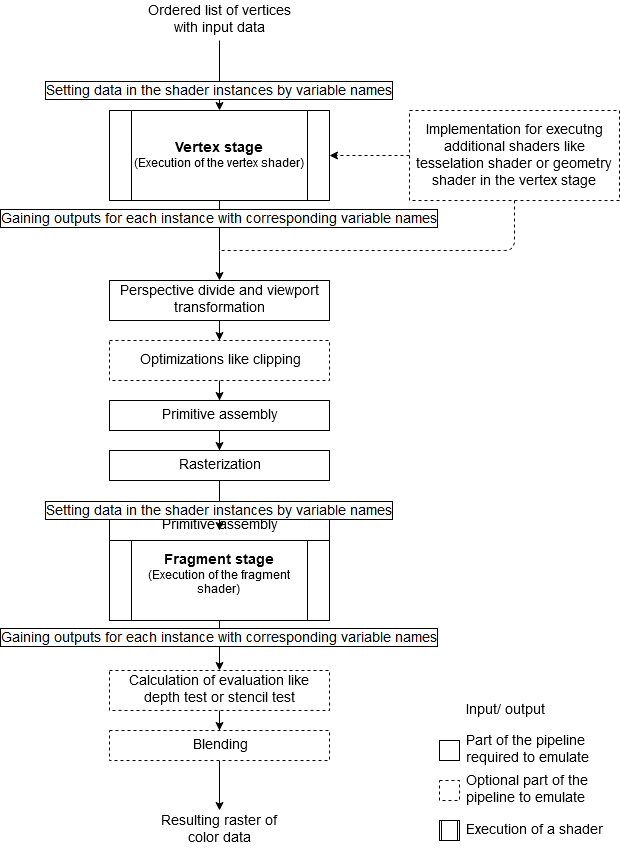
\includegraphics[scale=0.8]{infographic.png}
  \caption{Overview of the required steps to implement in the simulation}
  \label{fig:infographic}
\end{figure}


